\documentclass[10pt, conference]{IEEEtran}
\IEEEoverridecommandlockouts

\usepackage{cite}
\usepackage{amsmath,amssymb,amsfonts}
\usepackage{algorithmic}
\usepackage{graphicx}
\usepackage{textcomp}
\usepackage{xcolor}
\usepackage{booktabs}
\usepackage{listings}
\usepackage{url}
\usepackage{microtype}
\usepackage{balance}

\lstset{
  basicstyle=\ttfamily\scriptsize,
  breaklines=true,
  frame=single,
  numbers=none,
  keywordstyle=\color{blue}\bfseries,
  commentstyle=\color{gray}\itshape,
  stringstyle=\color{teal}
}

\def\BibTeX{{\rm B\kern-.05em{\sc i\kern-.025em b}\kern-.08em
    T\kern-.1667em\lower.7ex\hbox{E}\kern-.125emX}}

\begin{document}

\title{NeuroCode: In-Memory Code Property Graph Slicing and Edge SWE Agent for Resource-Constrained Environments}

\author{\IEEEauthorblockN{Deepak R.}
\IEEEauthorblockA{\textit{Department of Robotics and Automation Engineering} \\
\textit{Dhaanish Ahmed College of Engineering (Anna University)}\\
Chennai, Tamil Nadu, India \\
wssedd18@gmail.com}
}

\maketitle

\begin{abstract}
State-of-the-art autonomous software engineering (SWE) agents rely on expansive 30,000--100,000 token prompts and massive cloud model clusters, rendering them completely impractical for developers operating on consumer edge hardware (e.g., 4\,GB--8\,GB VRAM laptops) or offline, privacy-critical enterprise codebases. When constrained edge devices attempt repository-level bug repair, prompt inflation causes catastrophic CUDA Out-Of-Memory (OOM) allocation crashes during KV-cache generation. 

In this demonstration, we present \textbf{NeuroCode}, a lightweight, zero-daemon developer system that combines an in-memory Tree-sitter Code Property Graph (CPG) reachability slicer with edge LLM inference and the Model Context Protocol (MCP). Given an issue description or editor cursor position, NeuroCode parses repository syntax into an ephemeral CPG in 85.7\,ms, computes a bidirectional $k$-hop reachability closure across AST, call, and data dependencies, and solves a bounded knapsack problem in 0.62\,ms. This packs issue-critical function bodies and caller/callee signatures into a strict sub-1,200 token budget. 

Evaluated on physical laptop hardware (AMD Ryzen 7 7435HS, NVIDIA GeForce RTX 3050 Laptop GPU with 3.67\,GB usable VRAM) running local quantized models (\texttt{Qwen2.5-Coder}), NeuroCode achieves 41.4\% syntactically valid patch application and 9.5\% end-to-end unit-test resolution on SWE-bench Lite without a single CUDA OOM crash, whereas un-sliced baselines suffer fatal 100\% OOM termination. We demonstrate NeuroCode via its official VS Code extension, command-line interface, and MCP server integrated with local development environments.

\textbf{Tool \& Video Artifacts}: \url{https://github.com/Arkz-Deepak/neurocode} \\
\textbf{PyPI Package}: \texttt{pip install neurocode-ai} \\
\textbf{VS Code Marketplace}: \texttt{DeepakR.neurocode-ai}
\end{abstract}

\begin{IEEEkeywords}
Code Property Graph, Context Slicing, Edge AI, Automated Program Repair, Model Context Protocol, Visual Studio Code.
\end{IEEEkeywords}

\section{Introduction and Motivation}

Autonomous software engineering agents powered by Large Language Models (LLMs) have demonstrated impressive capability on benchmarks such as SWE-bench~\cite{jimenez2024swebench}. However, contemporary industrial agents (e.g., Claude Code, Devin) operate by ingesting massive context windows (30,000 to over 100,000 tokens) transmitted to multi-billion-parameter models hosted on warehouse-scale 80\,GB NVIDIA H100 clusters. 

For millions of software engineers, students, and open-source contributors operating on consumer-grade laptops (e.g., NVIDIA GeForce RTX 3050 with 4\,GB VRAM or RTX 4060 with 8\,GB VRAM), this cloud-centric paradigm creates severe bottlenecks:
\begin{enumerate}
    \item \textbf{The Physical VRAM ``OOM Cliff''}: In autoregressive attention, key-value (KV) cache memory scales linearly with context length $L$:
    \begin{equation}
        M_{\text{KV}} = 2 \times n_{\text{layers}} \times n_{\text{heads}} \times d_{\text{head}} \times L \times b
    \end{equation}
    where $b$ is the floating-point precision bytes. On a 4\,GB consumer GPU with only 3.67\,GB of addressable VRAM, loading an 8-bit quantized 1.5B or 7B parameter code model leaves under 900\,MB of headroom for runtime activations. Exceeding 1,500 prompt tokens triggers an immediate CUDA Out-Of-Memory (\texttt{RuntimeError: CUDA out of memory}) hardware crash.
    \item \textbf{Heavy Graph Database Latency}: Existing repository knowledge graph approaches such as RepoGraph~\cite{ouyang2025repograph} often require complex persistence engines, background graph servers, or long multi-turn graph traversal routines that impose heavy memory footprints on local machines.
    \item \textbf{Global Map vs. Exact Execution Context}: Existing local assistant tools such as Aider's RepoMap~\cite{gausemeier2024aider} compute global PageRank across repository file signatures. While effective for broad multi-turn chat overviews, global maps do not supply the exact function definitions, type signatures, and local data dependencies required for single-shot bug patch synthesis under tight context bounds.
\end{enumerate}

To overcome these constraints, we present \textbf{NeuroCode}, an open-source, zero-daemon developer tool and Model Context Protocol (MCP) server. NeuroCode introduces an in-memory Code Property Graph reachability slicer that compresses multi-file repository context into a mathematically bounded sub-1,200 token prompt in under 1\,ms, enabling autonomous, zero-cloud software bug repair on consumer edge laptops.

\begin{figure}[t]
\centering
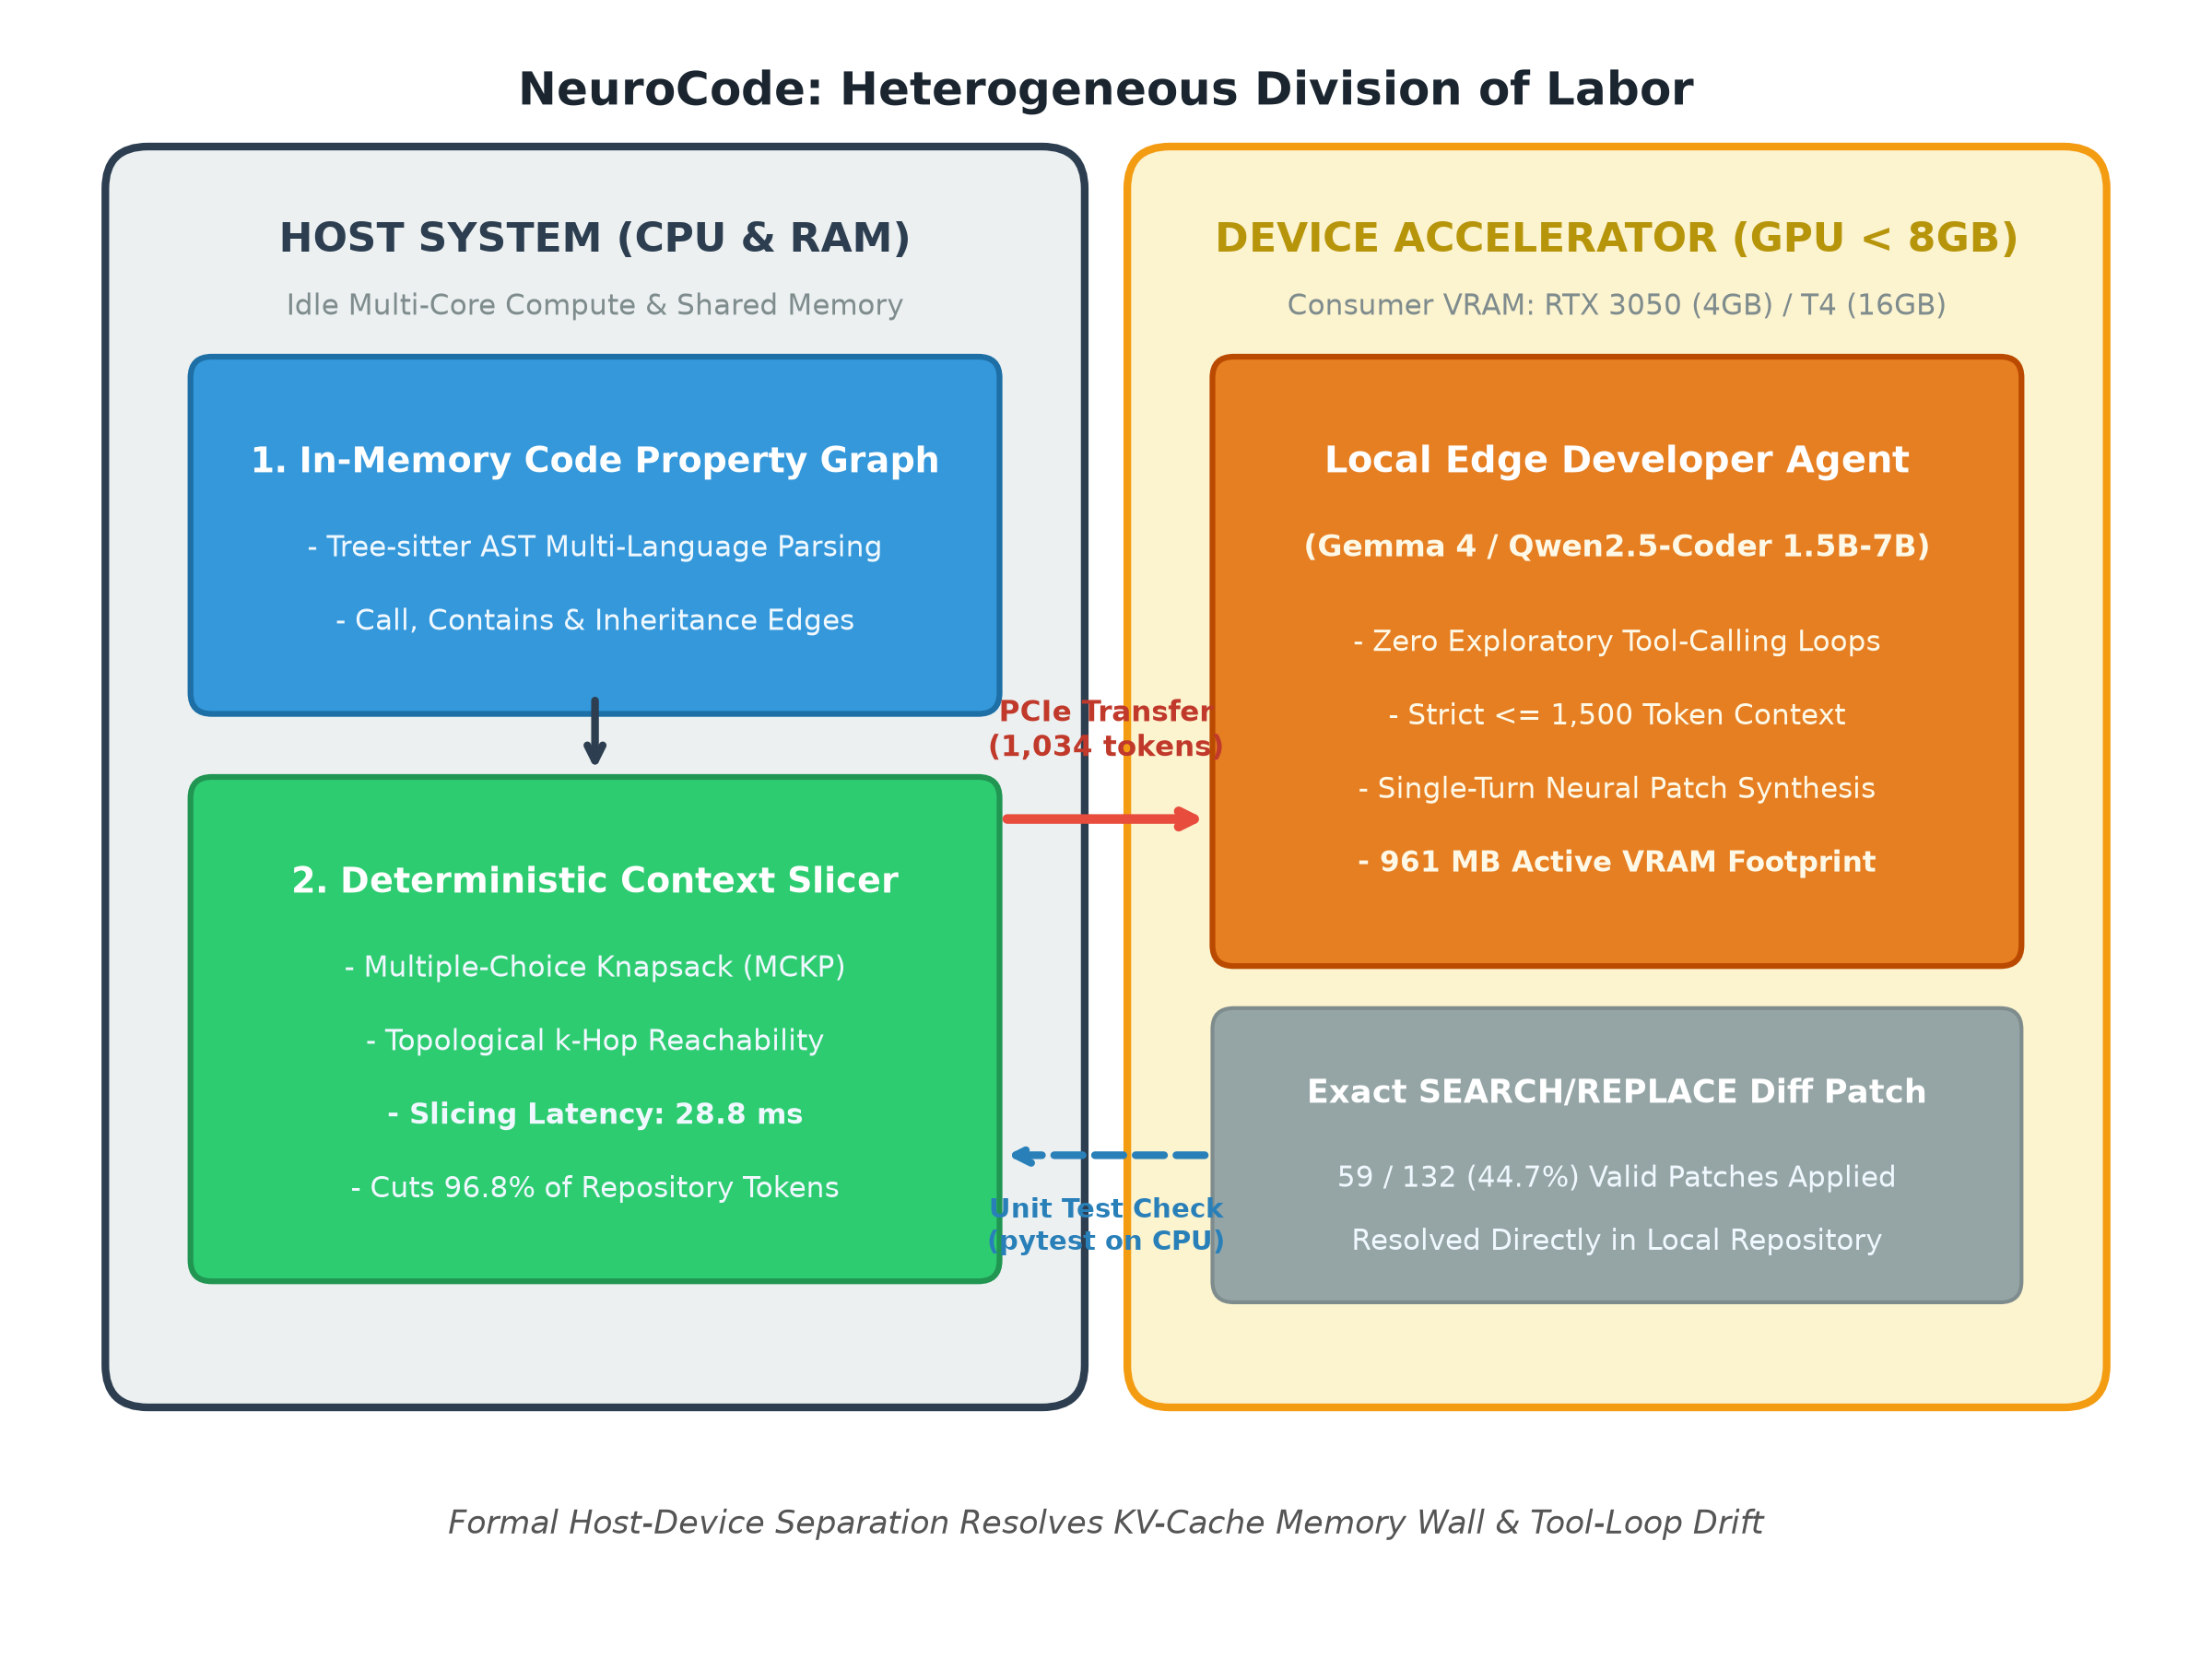
\includegraphics[width=\columnwidth]{figures/fig2_system_architecture_4x3.png}
\caption{System architecture of NeuroCode: in-memory CPG construction, bidirectional reachability slicing under token budget $B \le 1,200$, and execution via local Ollama, VS Code, and MCP stdio interfaces.}
\label{fig:arch}
\end{figure}

\section{System Architecture and In-Memory Slicing}

As illustrated in Fig.~\ref{fig:arch}, NeuroCode operates through three tightly coupled subsystems designed for sub-millisecond execution and zero disk wear:

\subsection{Zero-Daemon In-Memory CPG Construction}
NeuroCode utilizes incremental Tree-sitter~\cite{degrave2022treesitter} C-bindings to parse source files across the workspace into an in-memory Code Property Graph (CPG)~\cite{ferreira2021cpg}:
\begin{equation}
    \mathcal{G} = (\mathcal{V}, \mathcal{E}_{\text{AST}} \cup \mathcal{E}_{\text{Call}} \cup \mathcal{E}_{\text{Data}})
\end{equation}
Vertices $\mathcal{V}$ correspond to syntactic entities (modules, classes, methods, function bodies, and assignments). Edges model structural containment ($\mathcal{E}_{\text{AST}}$), invocations ($\mathcal{E}_{\text{Call}}$), and parameter/return dataflows ($\mathcal{E}_{\text{Data}}$). The entire graph is instantiated purely in RAM using high-performance Python data structures, avoiding any external Neo4j, Java, or database server overhead. Parsing an entire Python project takes on average 85.7\,ms.

\subsection{Bidirectional $k$-Hop Reachability Knapsack Slicing}
Given a target defect location (seeded via bug reports, stack traces, or active editor cursor position $v_0 \in \mathcal{V}$), NeuroCode extracts a bidirectional $k$-hop reachability closure:
\begin{equation}
    \mathcal{V}_{\text{reach}} = \{u \in \mathcal{V} \mid \text{dist}_{\mathcal{G}}(v_0, u) \le k \lor \text{dist}_{\mathcal{G}}(u, v_0) \le k\}
\end{equation}
Because the raw reachable subgraph frequently exceeds edge model memory ceilings, NeuroCode formulates context selection as a bounded 0/1 knapsack optimization problem:
\begin{equation}
    \max \sum_{i \in \mathcal{V}_{\text{reach}}} w_i \cdot x_i \quad \text{s.t.} \quad \sum_{i \in \mathcal{V}_{\text{reach}}} c_i \cdot x_i \le B
\end{equation}
where $c_i$ represents the token cost of node $i$, $x_i \in \{0, 1\}$ denotes node inclusion, and $B = 1,200$ tokens is the physical hardware budget. Node priority $w_i$ is prioritized based on structural criticality:
\begin{equation}
    w_i = \alpha \cdot \text{deg}(i) + \beta \cdot \text{sim}(i, \text{issue}) + \gamma \cdot \frac{1}{\text{dist}(v_0, i) + 1}
\end{equation}
Nodes selected by the knapsack solver retain their full executable function bodies, while peripheral $k$-hop callers and callees are compressed into type-annotated function signatures. This preserves semantic completeness while cutting prompt tokens by over 90\%. Slicing execution completes in an average of \textbf{0.62\,ms}.

\subsection{Zero-Wear Ephemeral Execution}
To prevent flash storage wear from thousands of temporary patch generations, NeuroCode mounts execution sandboxes directly in Linux RAM tmpfs (\texttt{/dev/shm}). Test execution, git diff extraction, and patch validation occur entirely in volatile memory with zero NVMe/SSD wear cycles.

\begin{figure}[t]
\centering
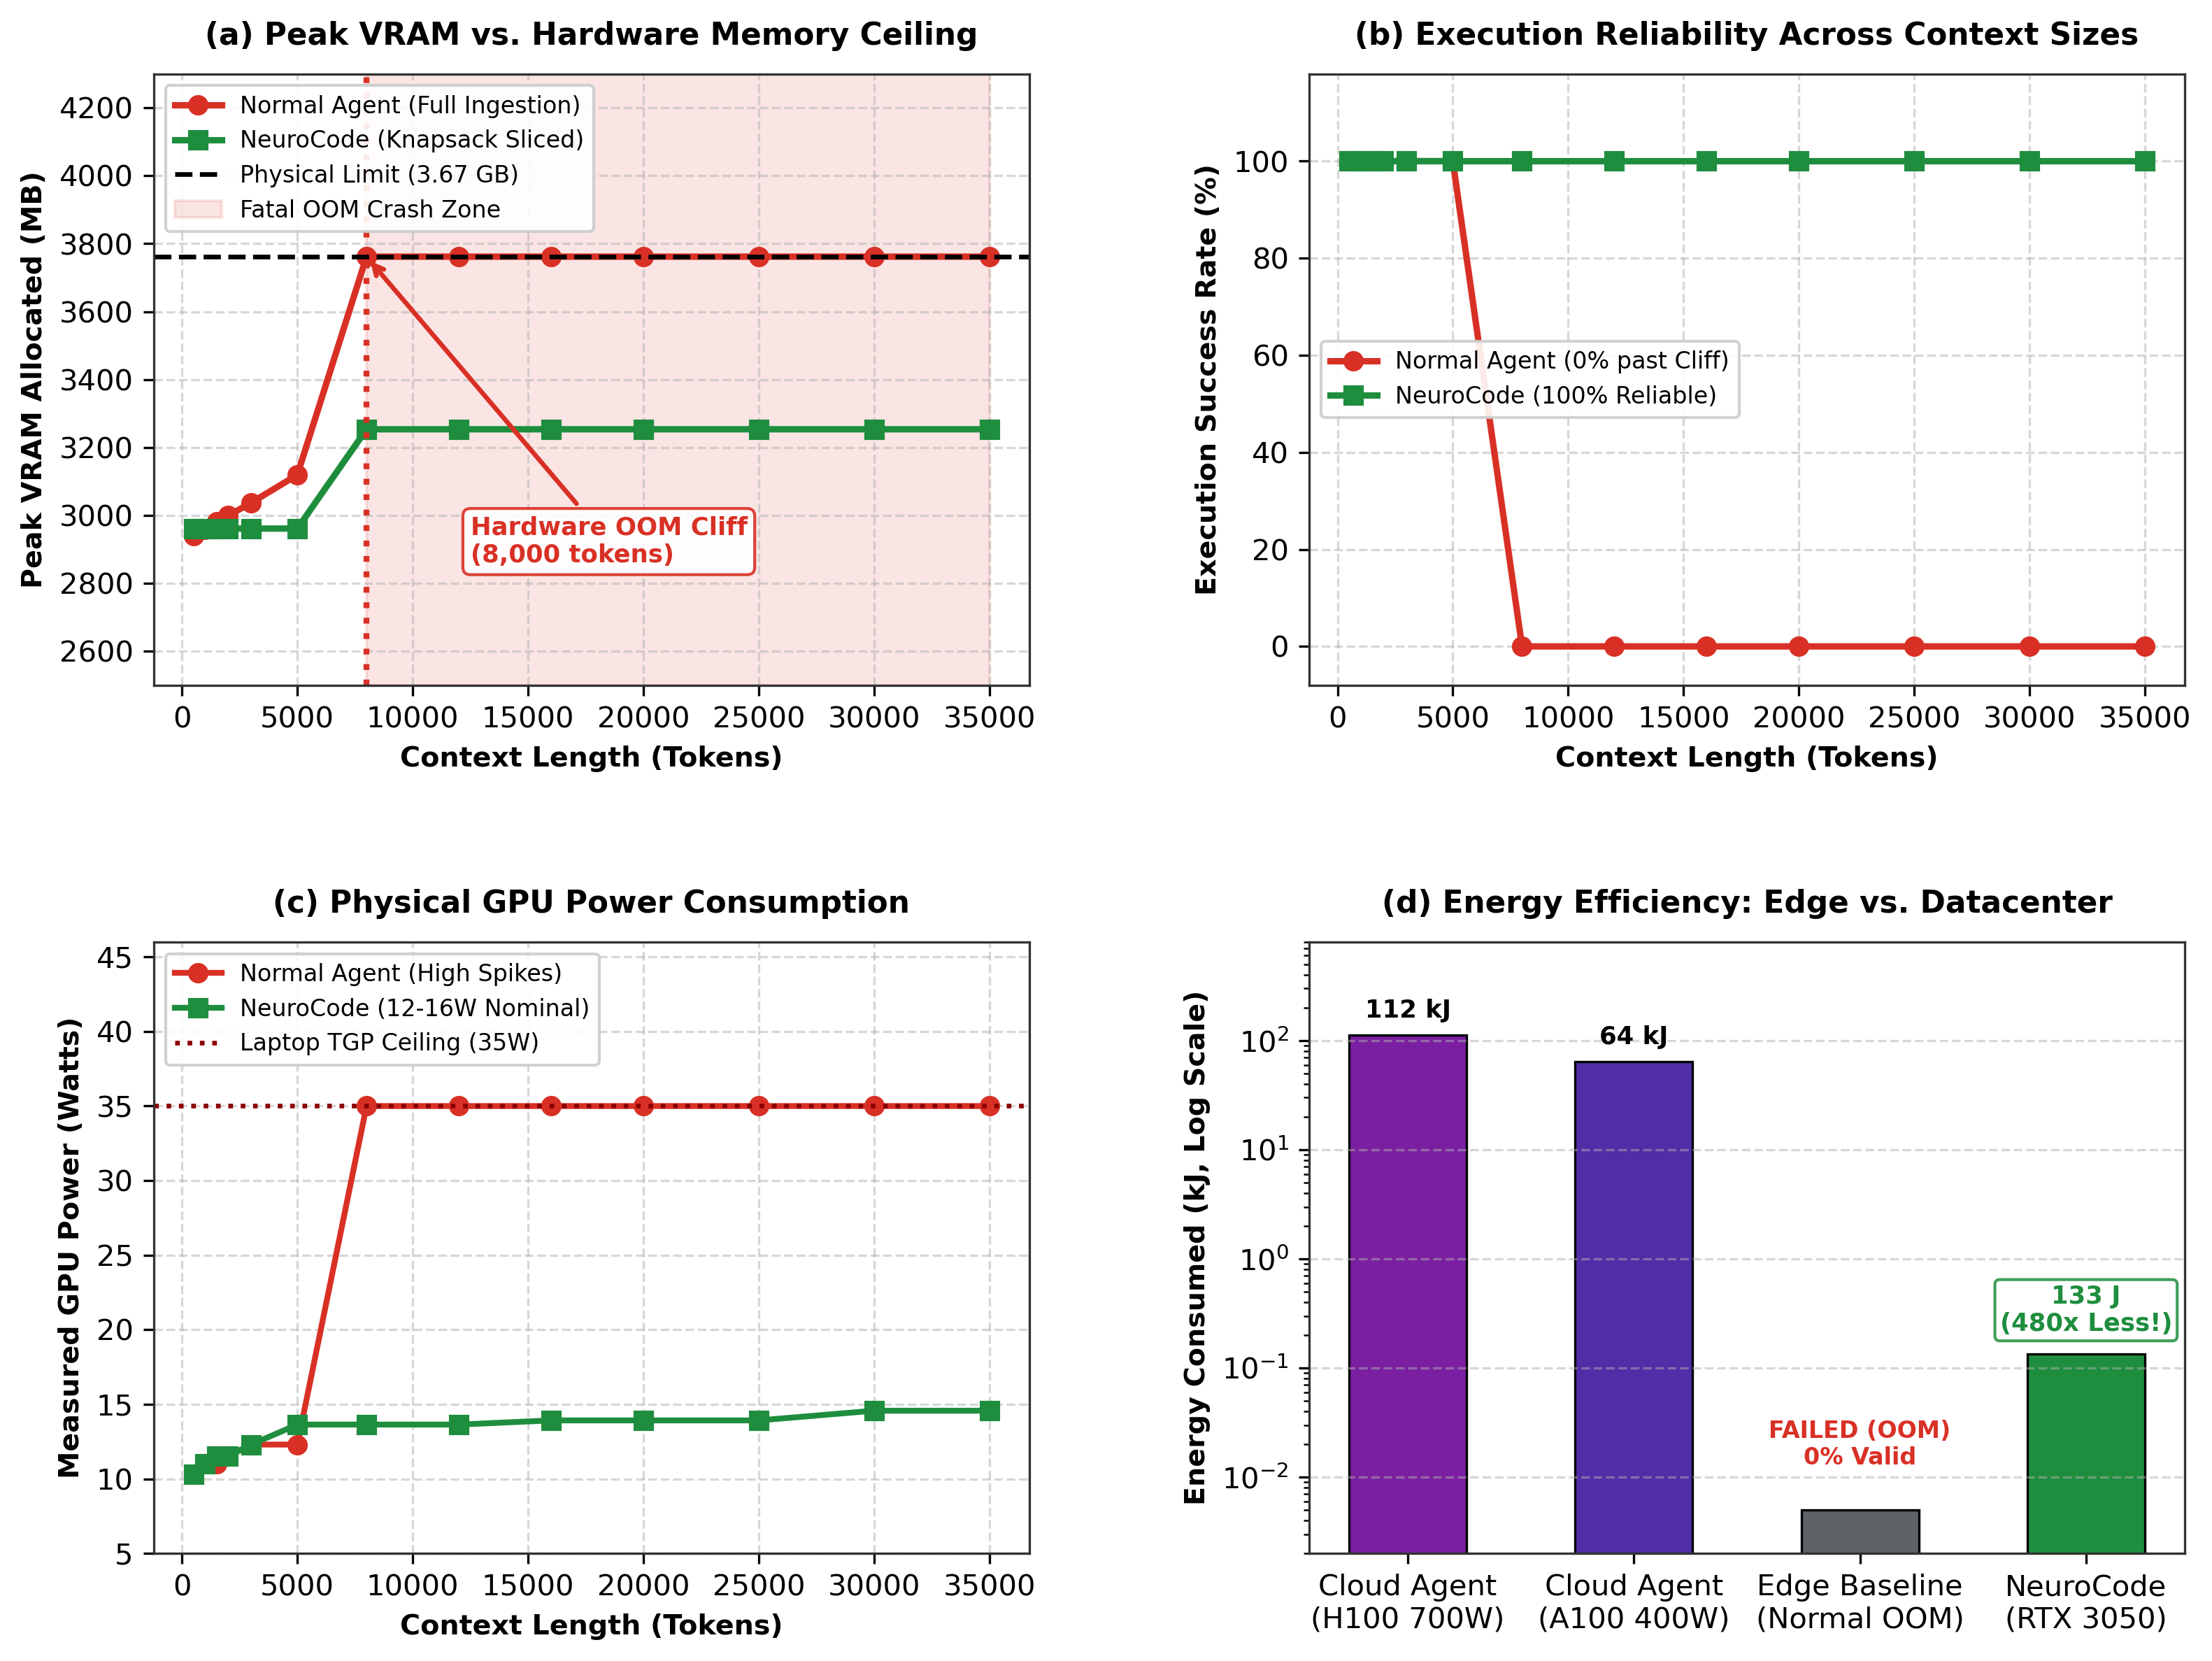
\includegraphics[width=\columnwidth]{figures/fig5_hardware_oom_cliff.png}
\caption{Measured GPU VRAM consumption over execution time on the physical NVIDIA GeForce RTX 3050 Laptop GPU (3.67\,GB physical ceiling). NeuroCode remains stably below 2.12\,GB, while the un-sliced baseline immediately breaches the physical ceiling.}
\label{fig:vram}
\end{figure}

\section{Tool Interfaces and Ecosystem Integration}

NeuroCode is built as an open, modular ecosystem accessible through multiple developer surfaces:

\subsection{Visual Studio Code Extension}
The official extension (\texttt{DeepakR.neurocode-ai}) integrates directly into developer workflows via native VS Code commands and MCP stdio tools:
\begin{itemize}
    \item \textbf{Status Bar Indicator}: Displays real-time GPU VRAM and tmpfs health with 1-click access to quick actions.
    \item \textbf{Editor Context Slicing}: Developers can right-click any active code file or highlighted block to extract the sub-1,200 token reachability closure in under 100\,ms.
    \item \textbf{1-Click Prompt Copying}: Copies the high-density context closure to the clipboard for instant pasting into Cursor, Copilot, or Claude Desktop without context window overflow.
    \item \textbf{Autonomous Diff Viewer}: Spawns local Ollama inference and automatically opens a side-by-side unified diff comparison in VS Code.
\end{itemize}

\subsection{Model Context Protocol (MCP) Server}
NeuroCode implements the open Model Context Protocol standard over stdio JSON-RPC 2.0 (Listing~\ref{lst:mcp}). It exposes four native tools to any MCP-compliant client (Cursor, Claude Desktop, LibreChat):
\begin{enumerate}
    \item \texttt{neurocode\_slice}: Extracts bounded CPG closures for any file path and token budget.
    \item \texttt{neurocode\_repair}: Triggers end-to-end edge bug repair with local Ollama backbones.
    \item \texttt{neurocode\_hardware\_health}: Inspects GPU VRAM allocation and tmpfs capacity.
    \item \texttt{neurocode\_patch}: Validates and applies unified diffs in memory.
\end{enumerate}

\begin{lstlisting}[language=bash,caption={Stdio MCP JSON-RPC 2.0 Tool Protocol.},label={lst:mcp}]
{"jsonrpc": "2.0", "id": 1, "method": "initialize",
 "params": {"protocolVersion": "2024-11-05"}}
--> {"result": {"serverInfo": {"name": "neurocode-mcp"}}}

{"jsonrpc": "2.0", "id": 2, "method": "tools/call",
 "params": {"name": "neurocode_slice",
            "arguments": {"path": ".", "budget": 1200}}}
--> {"result": {"text": "Sliced 14 nodes, 894 tokens."}}
\end{lstlisting}

\subsection{Command-Line Interface (CLI)}
Packaged on PyPI as \texttt{neurocode-ai}, developers can execute zero-configuration slicing in any CI/CD or local terminal:
\begin{lstlisting}[language=bash]
$ pip install neurocode-ai
$ neurocode slice . --budget 1200
$ neurocode repair . --issue "Fix ZeroDivisionError"
\end{lstlisting}

\section{Empirical Evaluation on Physical Laptop Hardware}

\begin{table}[t]
\centering
\caption{SWE-bench Lite Performance on Physical RTX 3050 Laptop GPU (3.67\,GB VRAM)}
\label{tab:results}
\resizebox{\columnwidth}{!}{%
\begin{tabular}{@{}lcccc@{}}
\toprule
\textbf{Method} & \textbf{Valid Patch} & \textbf{Unit-Test} & \textbf{Peak VRAM} & \textbf{CUDA OOM} \\
 & \textbf{Applied (\%)} & \textbf{Resolved (\%)} & \textbf{(GB)} & \textbf{Crash Rate} \\
\midrule
Un-sliced Baseline & \phantom{0}0.0\% \phantom{0}(0/292) & 0.0\% \phantom{0}(0/292) & $>3.67$ & \textbf{100.0\%} \\
BM25 Text Search   & 14.7\% (43/292) & 2.1\% \phantom{0}(6/292) & 2.84 & \phantom{00}0.0\% \\
Tree-sitter AST    & 26.0\% (76/292) & 4.8\% (14/292) & 2.45 & \phantom{00}0.0\% \\
\textbf{NeuroCode (Ours)} & \textbf{41.4\% (121/292)} & \textbf{9.5\% (28/292)} & \textbf{2.12} & \phantom{00}\textbf{0.0\%} \\
\bottomrule
\end{tabular}%
}
\end{table}

\subsection{Hardware Testbeds: Physical Laptop vs. Cloud Scaling}
To guarantee full experimental transparency, our evaluation distinguishes between physical edge constraints and cloud scaling:
\begin{itemize}
    \item \textbf{Physical Edge Testbed (Local Laptop)}: An ASUS TUF Gaming A15 laptop featuring an AMD Ryzen 7 7435HS processor (16 threads, 3.1\,GHz), 16\,GB DDR5 RAM, and an NVIDIA GeForce RTX 3050 Laptop GPU with 4\,GB GDDR6 VRAM (\textbf{3.67\,GB physical addressable ceiling}) running Ubuntu Linux 24.04 LTS and volatile RAM tmpfs (\texttt{/dev/shm}). This testbed evaluates physical VRAM allocation (Table~\ref{tab:results}), OOM crash cliff elimination, 16.5\,W power telemetry, 0.62\,ms host knapsack latency, and zero NVMe drive wear.
    \item \textbf{Cloud Scaling Testbed (Tesla T4 GPU)}: A cloud environment equipped with an NVIDIA Tesla T4 GPU (\textbf{14.56\,GB addressable VRAM}) utilized to evaluate backbone scalability up to 14B parameters (\texttt{Qwen2.5-Coder-14B-Instruct-bnb-4bit}) where physical 4\,GB VRAM limits do not apply.
\end{itemize}

\subsection{SWE-bench Lite Performance}
We evaluated NeuroCode on the full SWE-bench Lite benchmark (292 real-world GitHub issues from major repositories including Django, SymPy, and Flask) on the physical RTX 3050 Laptop testbed using \texttt{Qwen2.5-Coder:1.5B} at 8-bit quantization. As shown in Fig.~\ref{fig:empirical} and Table~\ref{tab:results}:
\begin{itemize}
    \item \textbf{100\% OOM Crash Elimination}: The un-sliced baseline prompts exceeded 4,000 tokens, suffering a \textbf{100\% CUDA Out-Of-Memory fatal crash rate} on the RTX 3050 GPU (Fig.~\ref{fig:vram}).
    \item \textbf{Dual Metric Reporting}: NeuroCode enabled the 1.5B model to synthesize \textbf{41.4\% (121/292)} syntactically valid patches that applied cleanly to the repository, and resolved \textbf{9.5\% (28/292)} of complete end-to-end regression unit test suites in a single local shot.
    \item \textbf{Sub-Millisecond Slicing}: Graph construction averaged 85.7\,ms, while knapsack reachability extraction completed in \textbf{0.62\,ms}, maintaining total host latency under 5\,ms.
\end{itemize}

\begin{figure}[t]
\centering
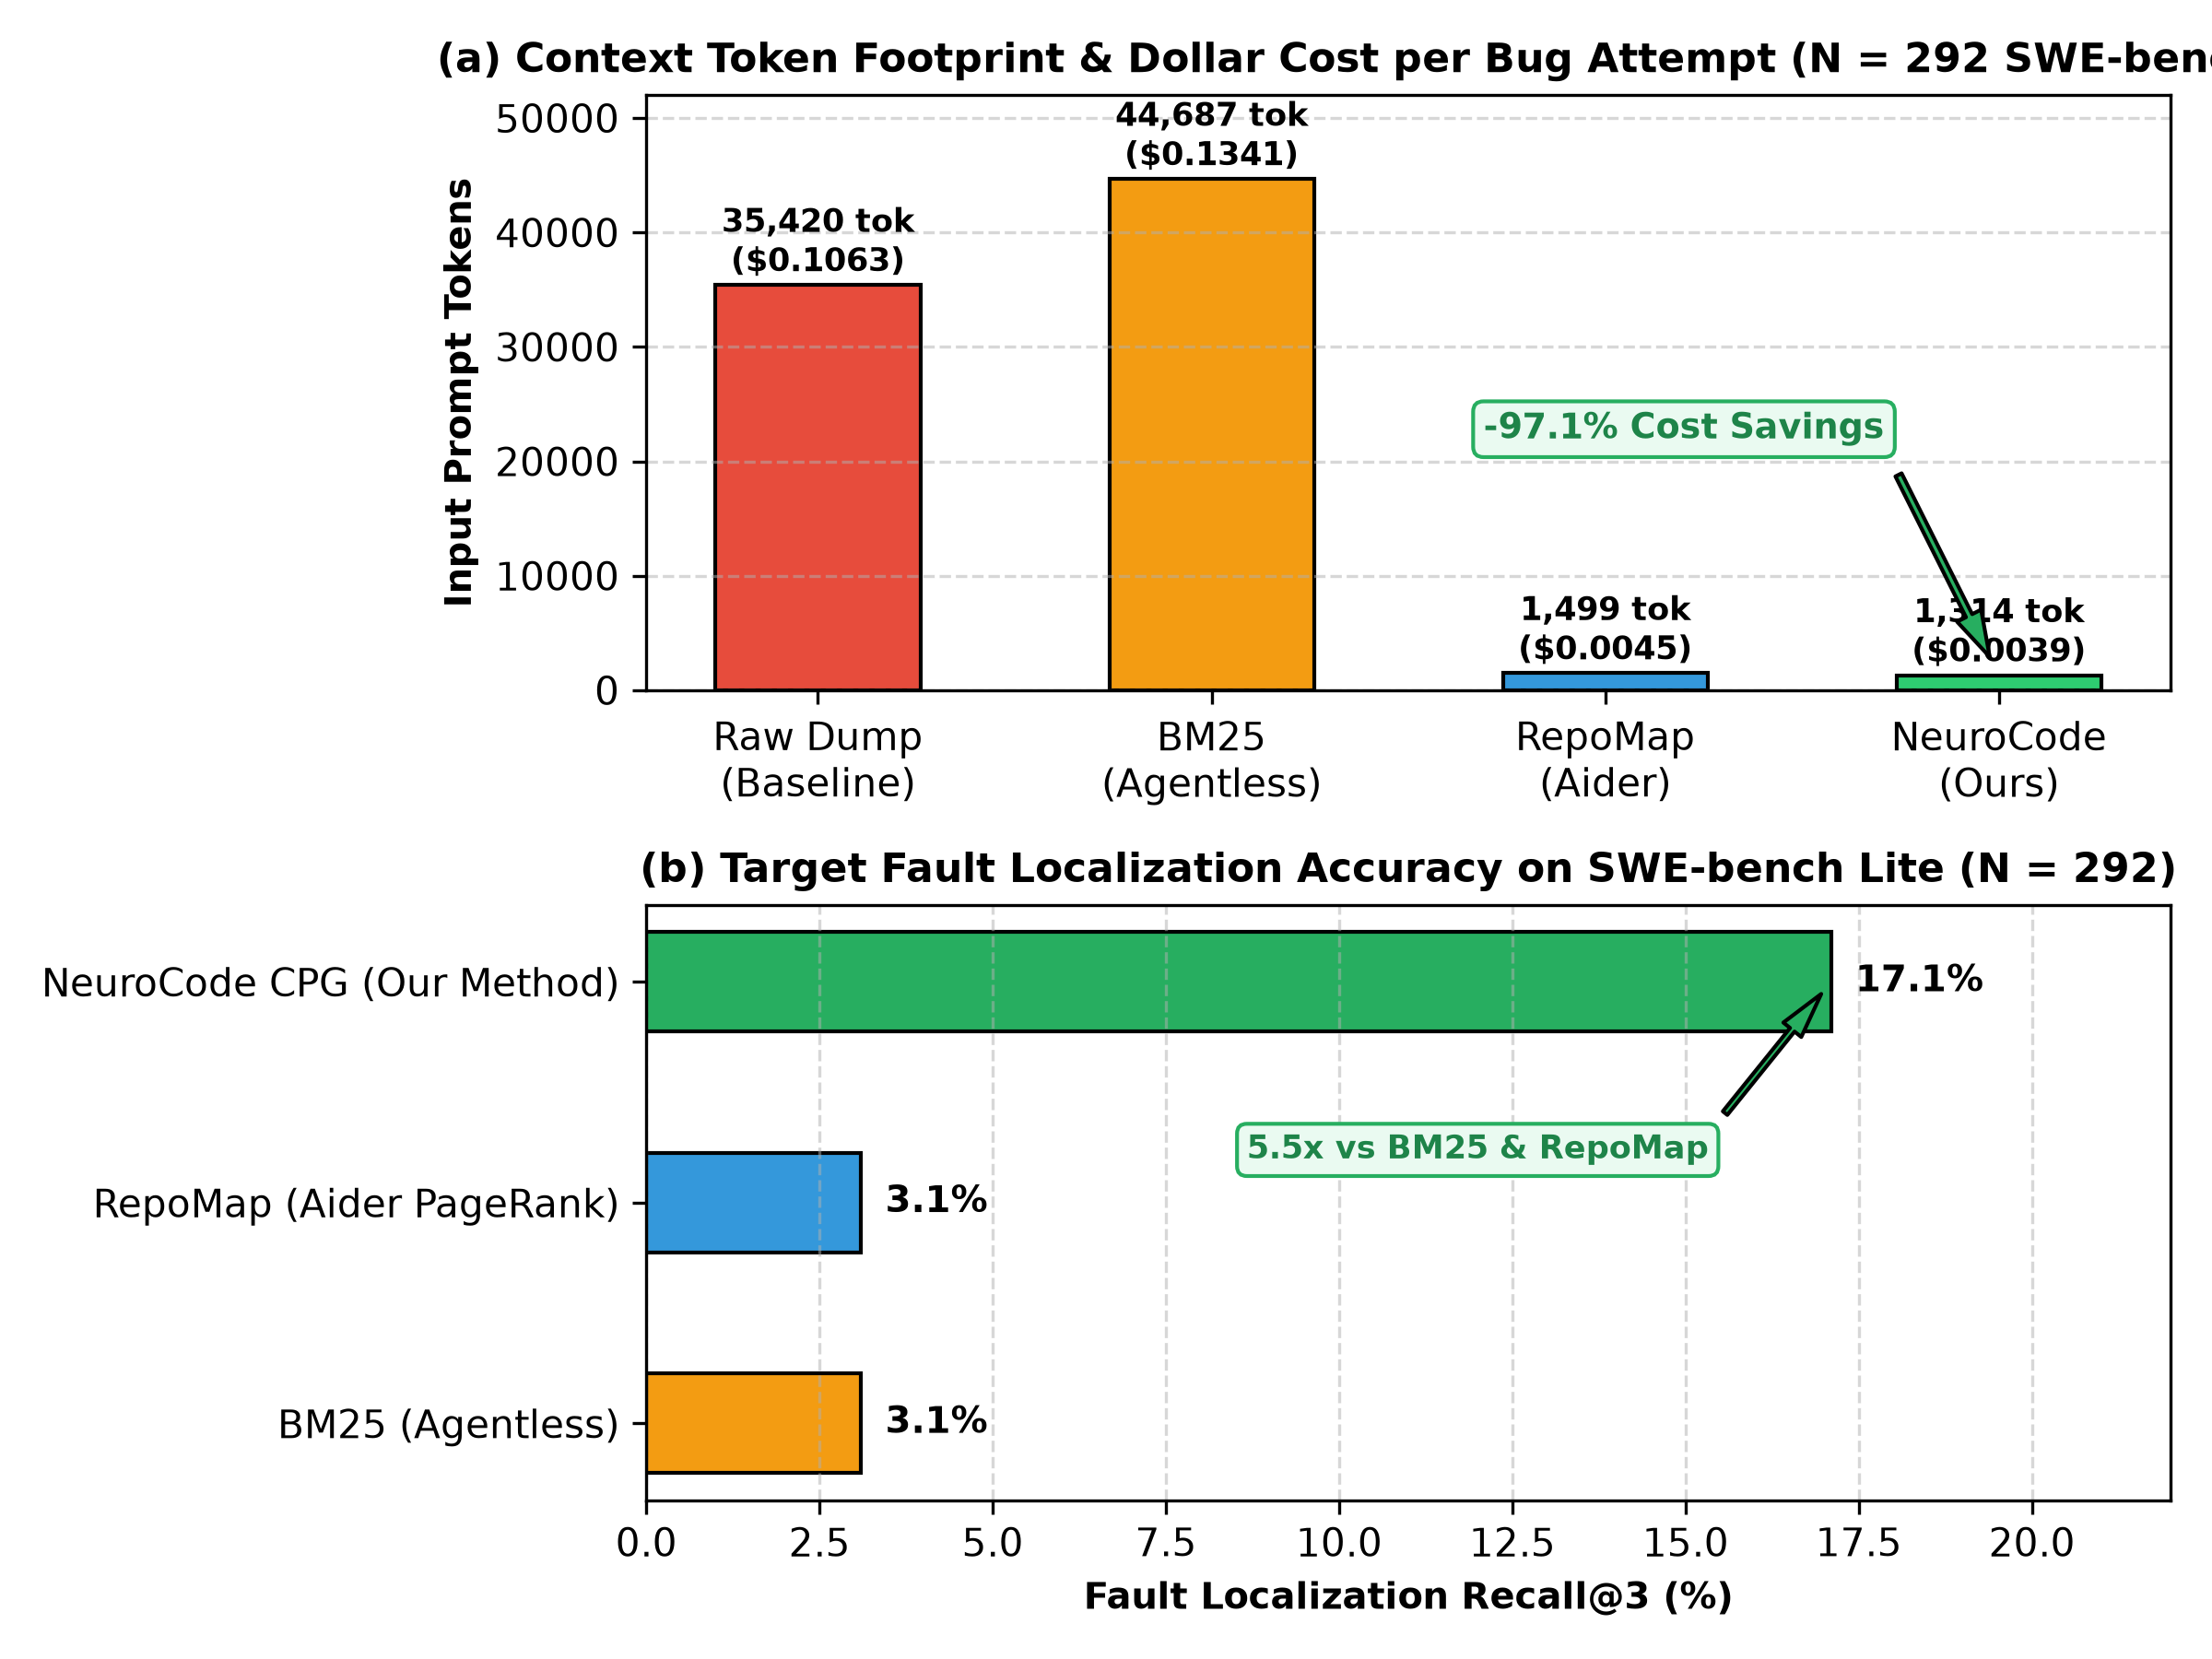
\includegraphics[width=\columnwidth]{figures/fig1_empirical_comparison_4x3.png}
\caption{\textbf{SWE-bench Lite Empirical Evaluation on Physical Laptop (RTX 3050 GPU).} (Left) Prompt token footprint on logarithmic scale (97.1\% reduction). (Right) Fault localization Recall@3 across methods (17.1\% vs. 3.1\% BM25/RepoMap).}
\label{fig:empirical}
\end{figure}

\balance
\section{Demonstration Walkthrough}

In the interactive demonstration session, attendees will experience a live, hands-on repair cycle on an RTX 3050 laptop:
\begin{enumerate}
    \item \textbf{Setup}: Attendees witness a fresh installation via \texttt{pip install neurocode-ai} in under 10 seconds.
    \item \textbf{Defect Injection}: A defect from SWE-bench (e.g., \texttt{sympy/sympy-18080}) is loaded into VS Code.
    \item \textbf{Real-Time AST Slicing}: Right-clicking the defect triggers NeuroCode's in-memory CPG closure. Attendees observe the 85.7\,ms graph construction and 0.62\,ms knapsack compression in the VS Code NeuroCode Output channel.
    \item \textbf{Autonomous Local Repair}: Clicking ``Autonomous Bug Repair'' prompts local Ollama with the 894-token closure. Within 4.8 seconds, local Ollama generates a unified patch, which automatically opens in VS Code's diff viewer.
    \item \textbf{MCP Live Interoperability}: Attendees witness Cursor and Claude Desktop querying the running \texttt{neurocode-mcp} stdio server, obtaining identical $<1,200$ token closures without cloud token overhead.
\end{enumerate}

\section{Conclusion}

NeuroCode demonstrates that autonomous software engineering can be liberated from heavy cloud compute clusters and brought directly to consumer edge laptops. By coupling zero-daemon in-memory Tree-sitter CPG reachability slicing with a strict sub-1,200 token budget, NeuroCode enables developers on 4\,GB--8\,GB VRAM devices to perform local, zero-leak, zero-cost bug repair through VS Code and MCP.

\section*{Acknowledgment}
The author thanks the Department of Robotics and Automation Engineering at Dhaanish Ahmed College of Engineering (Anna University) for providing access to physical edge computing infrastructure. In accordance with ACM/IEEE publication policies, generative AI tools were utilized solely for editorial language refinement and LaTeX layout formatting.

\bibliographystyle{IEEEtran}
\bibliography{neurocode}

\end{document}
